%Introductory sentences here
In this section, we describe how we generated a realistic simulated data set for dexterous grasping. This captures variations in both observable (e.g. object pose) and unobservable (e.g. surface friction) parameters.

To generate the training set a simulated depth image of a scene containing a single unfamiliar object is generated. Using the generative model, grasps are generated and executed in simulation. The success or failure of each simulated grasp is recorded. Producing a good simulation for evaluating grasps is non-trivial. An important problem is that the data set must capture the natural uncertainty in unobservable variables, such as mass and friction. This is related to domain randomisation. Domain randomisation can include unrealistic variations in appearance. Here, however, we only include variations within the known bounds of objects the robot may grasp. We thus refer to this as {\em robust evaluation}. A similar technique has been employed by \cite{mahler2017dex}, but we extend it from a grasp quality metric to full rigid body simulation.

\subsection{Features and Constraints of the Virtual Environment}
\label{subsection:environment}

We employ MuJoCo \cite{MuJoCo} as the rigid-body simulator. The dataset of 294 objects is drawn from 20 classes and includes: bottles, bowls, cans, boxes, kitchen utensils, mugs, cups, pans and other graspable objects such as tennis balls and dust pans (Figure \ref{fig:allObjects}). The number of objects in each class varies from 1 (dustpan) to 25 (bottles). 250 objects from all classes were used for training and 44 for testing. Long/thin objects are placed vertically in a short, heavy stand in order to make them graspable without touching the table. Due to the fact that collision checking in MuJoCo requires that objects comprise convex parts, all 294 objects were decomposed into convex parts \cite{V-HACD}. The number of sub-parts varies from 2 to 120. 

To achieve robust simulation, prior distributions for mass, size and frictional coefficient were estimated from real-world data. The properties of simulated objects are sampled from these priors. For each object its mean size, mass and friction coefficient are matched to a real counterpart. For each trial, the size is randomly scaled by a factor in the range [0.9,1.1], while remaining within the grasp aperture of the hand. Object mass is uniformly sampled from a category specific range, estimated from real objects (Table~\ref{fig:weights}). The friction coefficient of each object is sampled from a range of $[0.5, 1]$ in MuJoCo default units, intended to simulate surfaces from low-friction (metal) to high-friction (rubber). This variation is critical to ensuring that the evaluative model will predict the robustness of a grasp to unobservable variations.
\begin{table}[]
\centering
\caption{Mass ranges for each object class (grams).}
\label{fig:weights}
\resizebox{\linewidth}{!}{\begin{tabular}{|l|l|l|l|l|l|l|}
\hline
Bottle & Bowl     & Box     & Can     & Cup    & Fork    & Pan     \\ \hline
30-70  & 50-400   & 50-500  & 200-400 & 30-330 & 40-80   & 150-450 \\ \hline
Plate  & Scissors & Shaker  & Spatula & Spoon  & Teacup  & Teapot  \\ \hline
40-80  & 50-150   & 100-160 & 40-80   & 40-80  & 150-250 & 500-800 \\ \hline
Jug    & Knife    & Mug     & Funnel  & Ball   & Dustpan &         \\ \hline
80-200 & 50-150   & 250-350 & 40-80   & 50-70  & 100-150 &         \\ \hline
\end{tabular}}
\end{table}
 
For depth image simulation the Carmine 1.09 depth sensor installed on the robot is simulated with a modified version of the Blensor Kinect sensor simulator \cite{KinectSimulator}. For each object, we vary the camera orientation and distance from the object, as well as object mass, friction, scale, location and orientation. 

A 3D mesh-model of the DLR-II hand has been used in the simulator. There are no kinematic constraints on how the hand may grasp an object, other than collisions with the table. To ensure realism, we use impedance control for the hand.
%The reasons for the most critical of these decisions are now given in slightly more detail. First, in order to create a realistic simulation environment, we chose the MuJoCo \cite{MuJoCo} physics simulator over other simulators (OpenSim, BulletPhysics, ODE, NVIDIA PhysX) for two reasons: 
%\begin{itemize}
%\item MuJoCo uses generalized coordinates and optimization-based contact dynamics, resulting in fewer numerical instabilities,
%\item MuJoCo is optimized for the quality of physics as well as its speed, hence improving the quality of the physics simulation.
%\end{itemize}
%\begin{figure}
%  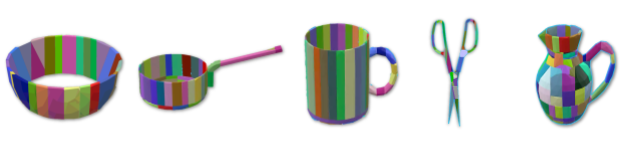
\includegraphics[width=\linewidth]{images/decomposition.png}
%  \caption{Approximate convex decomposition of some objects in our dataset. Best viewed in colour.}
%  \label{fig:objectDecomposition}
%\end{figure}

\subsection{Data Collection Methodology}
\label{subsection:dataCollection}

The data set is divided into units called \textit{scenes}, where each scene comprises a single object placed on a table. Many grasps are attempted per scene. Below, we specify the time flow of data collection:

\begin{enumerate}
\item A novel instance of an object from the dataset is generated and placed on a virtual table. Variations are applied to object pose, scale, mass, and friction coefficient.
\item A simulated camera takes a depth image $I_s$ of the scene, converted to a point cloud $P_s$. The viewpoint ${elevation}_s$ of the view point is from 30-57 degrees. The ${azimuth}_s$ is sampled from $[0, 2\pi]$. 
\item The generative model proposes 100 candidate grasps. These are the 10 grasps that are highest ranked by the GM for each of the 10 training grasps. These are applied to the object in simulation.
\item 20 further simulated depth images are taken from other viewpoints around the object, as explained in step 2. Images with fewer than 250 depth points are discarded. We then sample with replacement from the remaining images and associate each sampled image and viewpoint with a grasp created in step 3.
\item The grasp outcome, trajectory and depth image are stored for each trial. The grasp parameters are converted to the camera frame for the associated view.
\end{enumerate}

%Each candidate grasp $h_i = \{w_0, ..., w_{n}\}$ consists of a series of 10 waypoints along : $w_0$, ..., $w_{n}$. A waypoint $w_k$ is a 27-element vector that specifies full configuration of the hand in joint space: 3 dimensions for 3D coordinates and 4 dimensions for the orientation of the wrist, and 20 parameters specifying each finger joint's activation. 
%After a grasp $h_i$ is generated in world coordinates, the waypoints that belong to the grasp are converted to the camera's frame of reference. 
%The goal of our network architecture is to learn which grasps are more likely to succeed given a point cloud, where both input channels are represented in terms of the camera frame of reference. %This point differentiates us from the work of Levine et al. \cite{Levine1}, where camera coordinates are not used. It should be noted that the possible camera locations in our simulated data covers a larger space, with full circular movement $[0, 2\pi]$ on azimuth and $[30-57]$ range in elevation. Our scenes do not have any distinguishing landmarks such as a bin or robot base, which may aid the network in locating the camera in the scene. 

In each scene $S_i$, a number of depth images are taken $\{I_{ik}\}_{k=0}^{20}$, in the manner explained above. The first image $I_{i0}$ is used to generate grasps, as explained in Section \ref{section:generative}. We typically perform 100 grasps per scene. Attaching different views to each grasp instead of the seed image $I_{i0}$ ensures there is more variation in terms of viewpoints, resulting in a richer dataset. Typically, performing a grasp takes half the time it takes to acquire an image using the simulated camera.

Once a grasp is performed in simulation, it is considered a success if an object is lifted one metre above the table, and held there for two seconds. If the object slips from the hand during lifting or holding, the grasp is a failure. 

\begin{figure}[t]
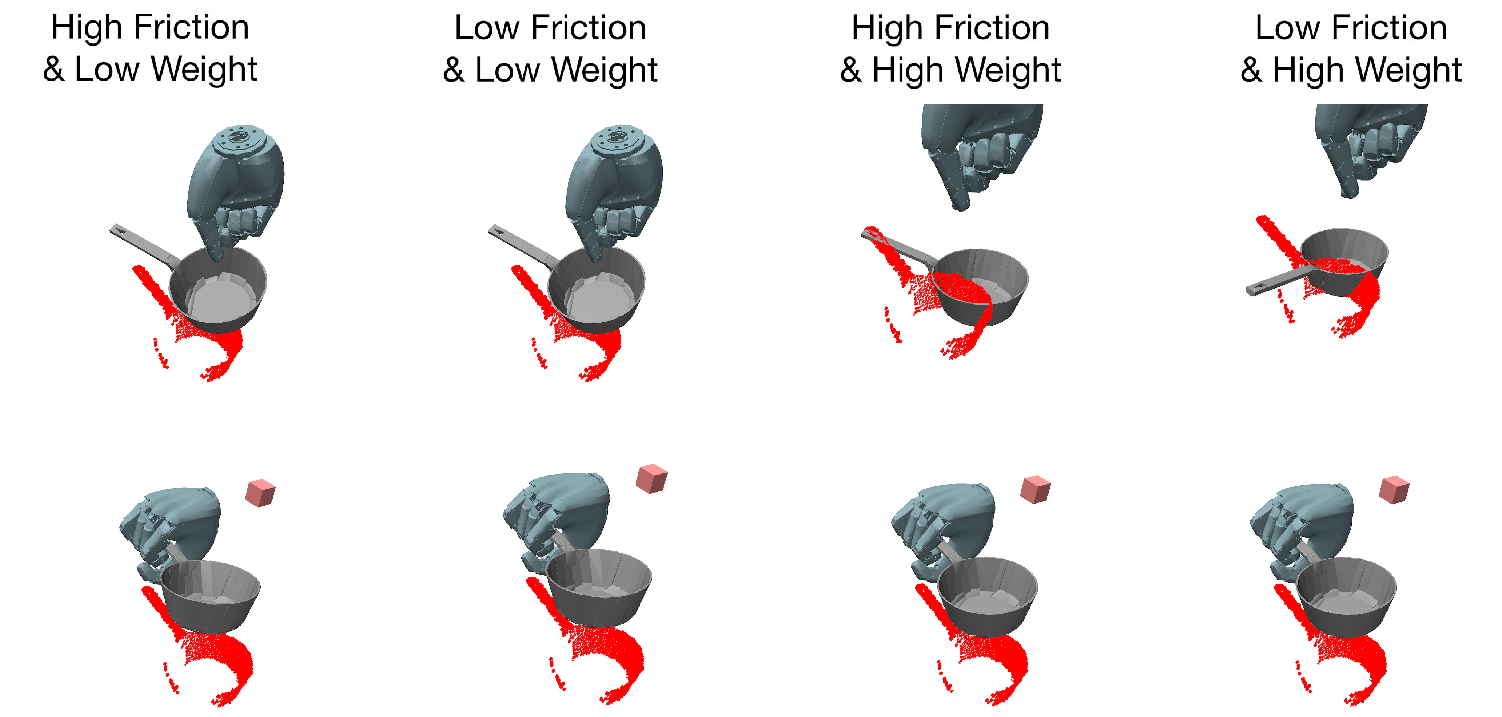
\includegraphics[width=\columnwidth]{images/frictionweight}
%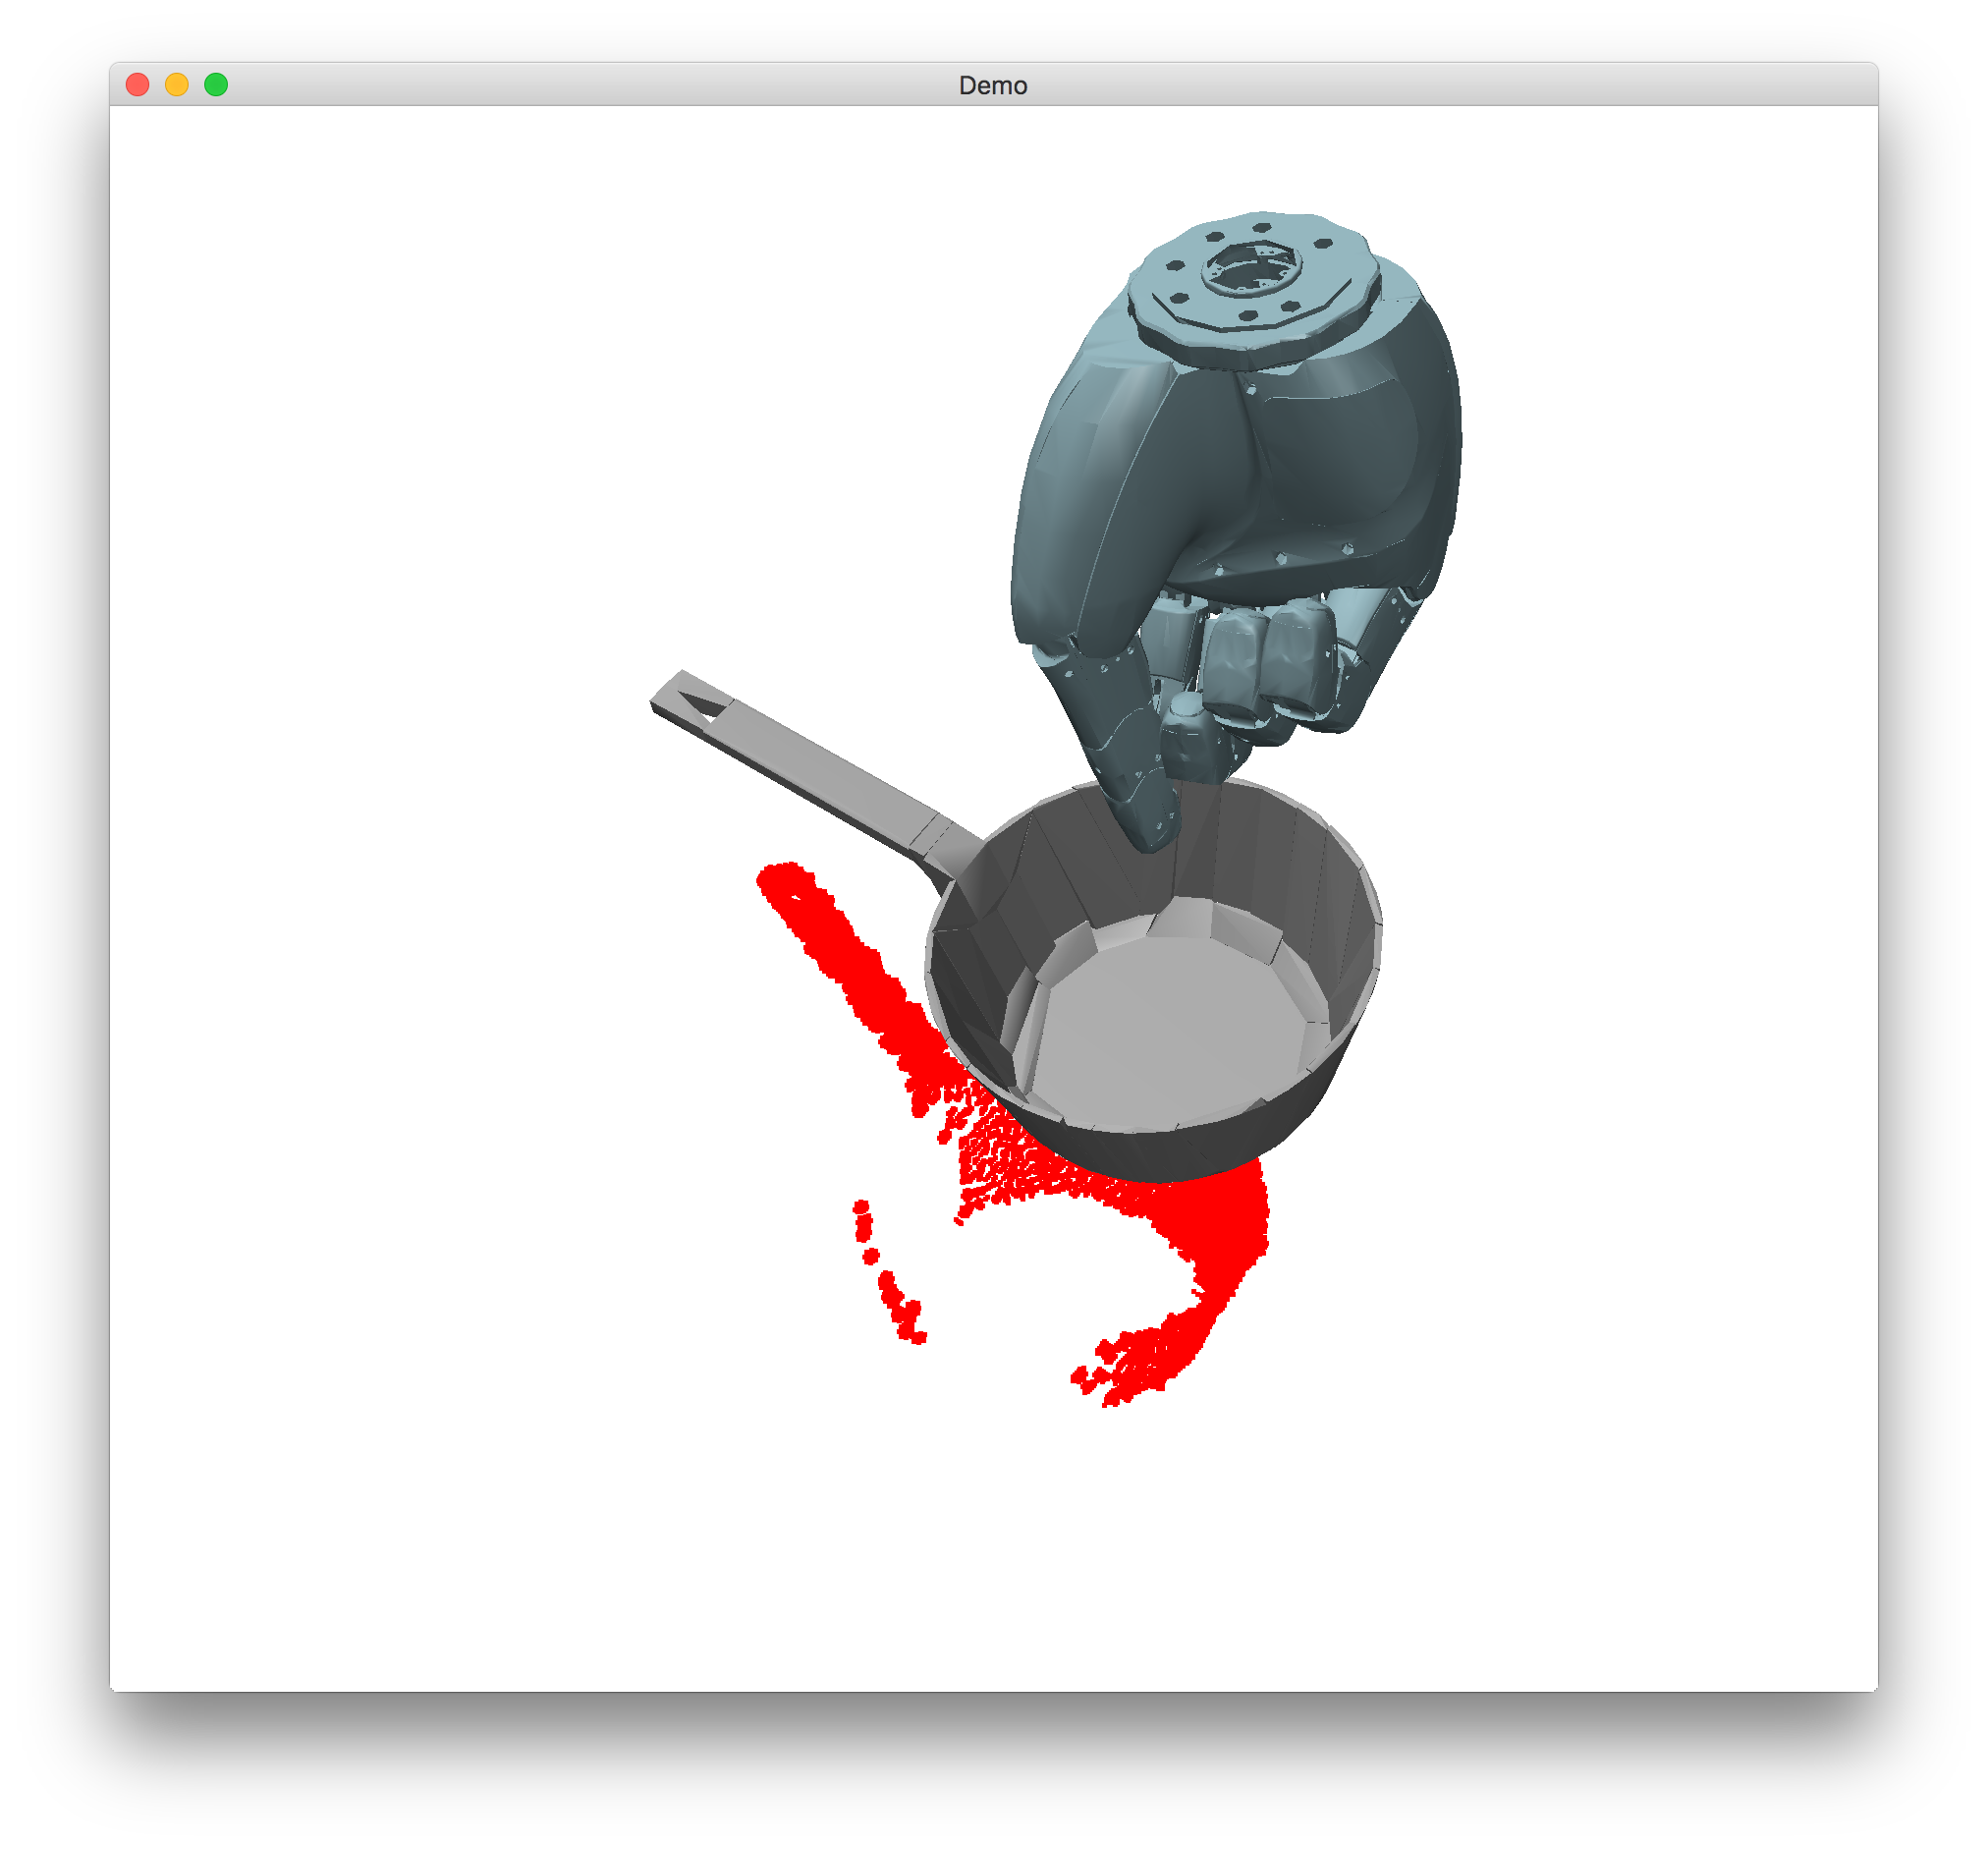
\includegraphics[width=0.24\textwidth]{images/Pan4_2_HFLW}
%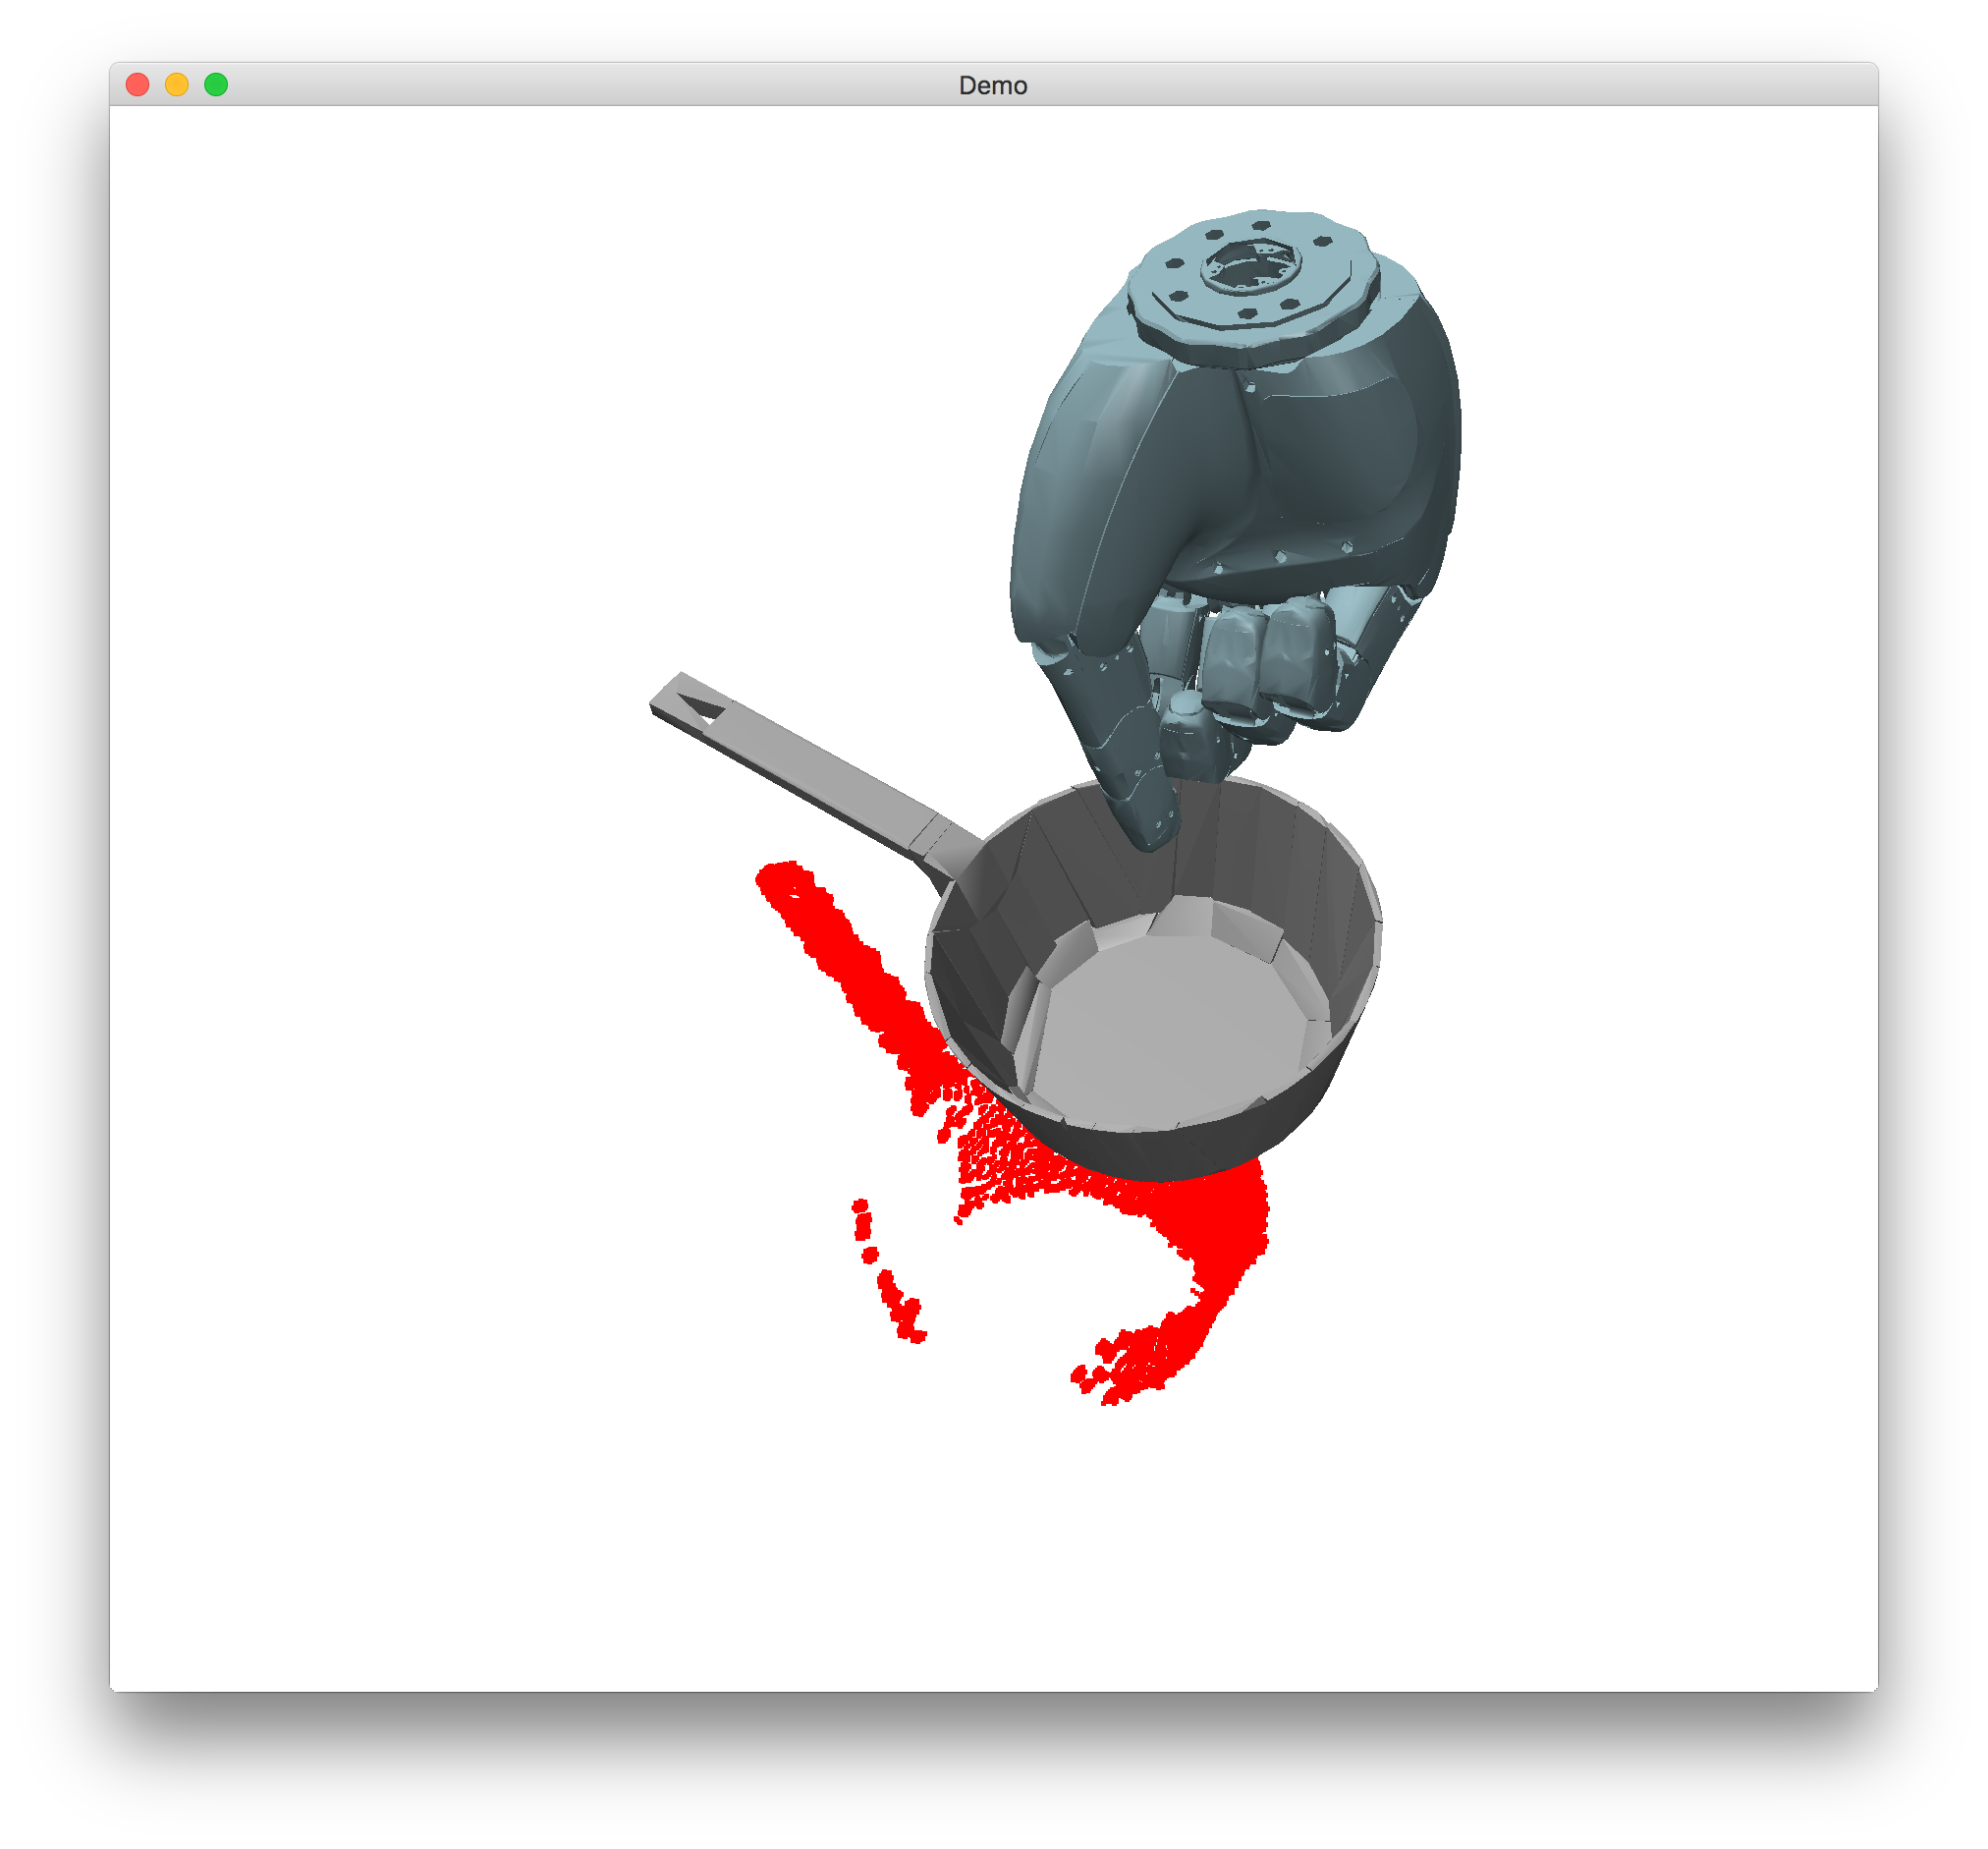
\includegraphics[width=0.24\textwidth]{images/Pan4_2_LFLW}
%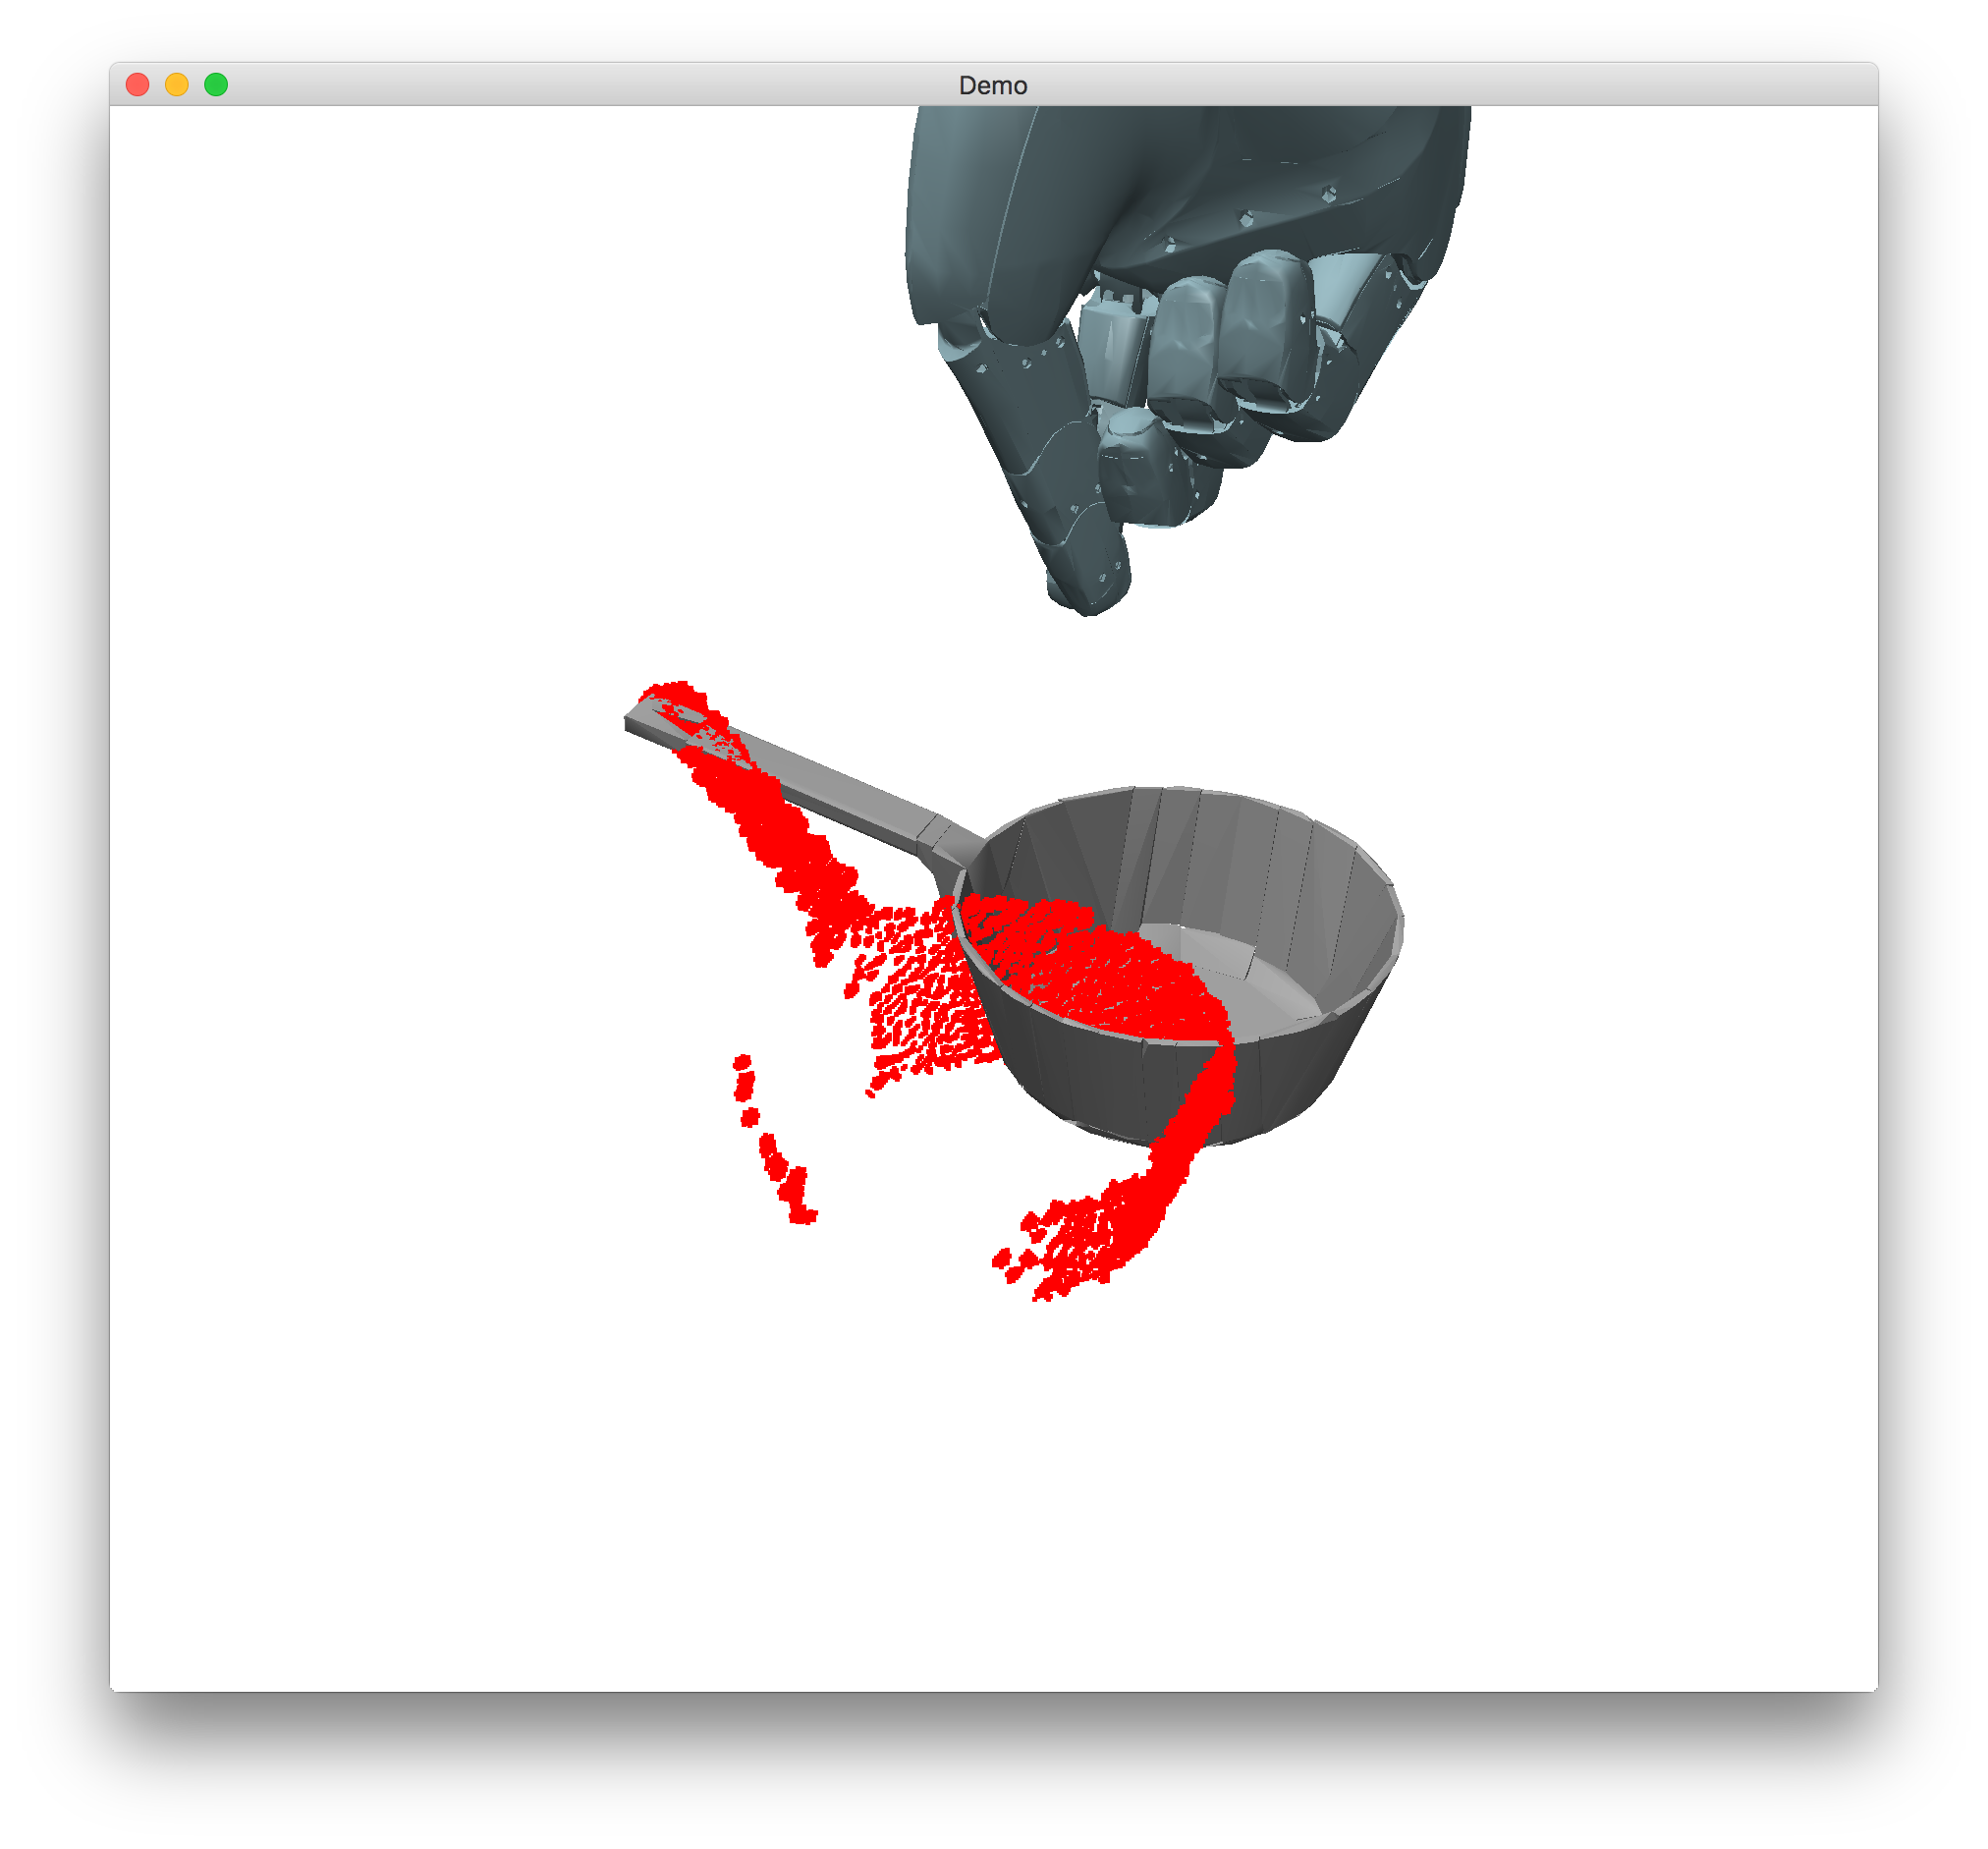
\includegraphics[width=0.24\textwidth]{images/Pan4_2_HFHW}
%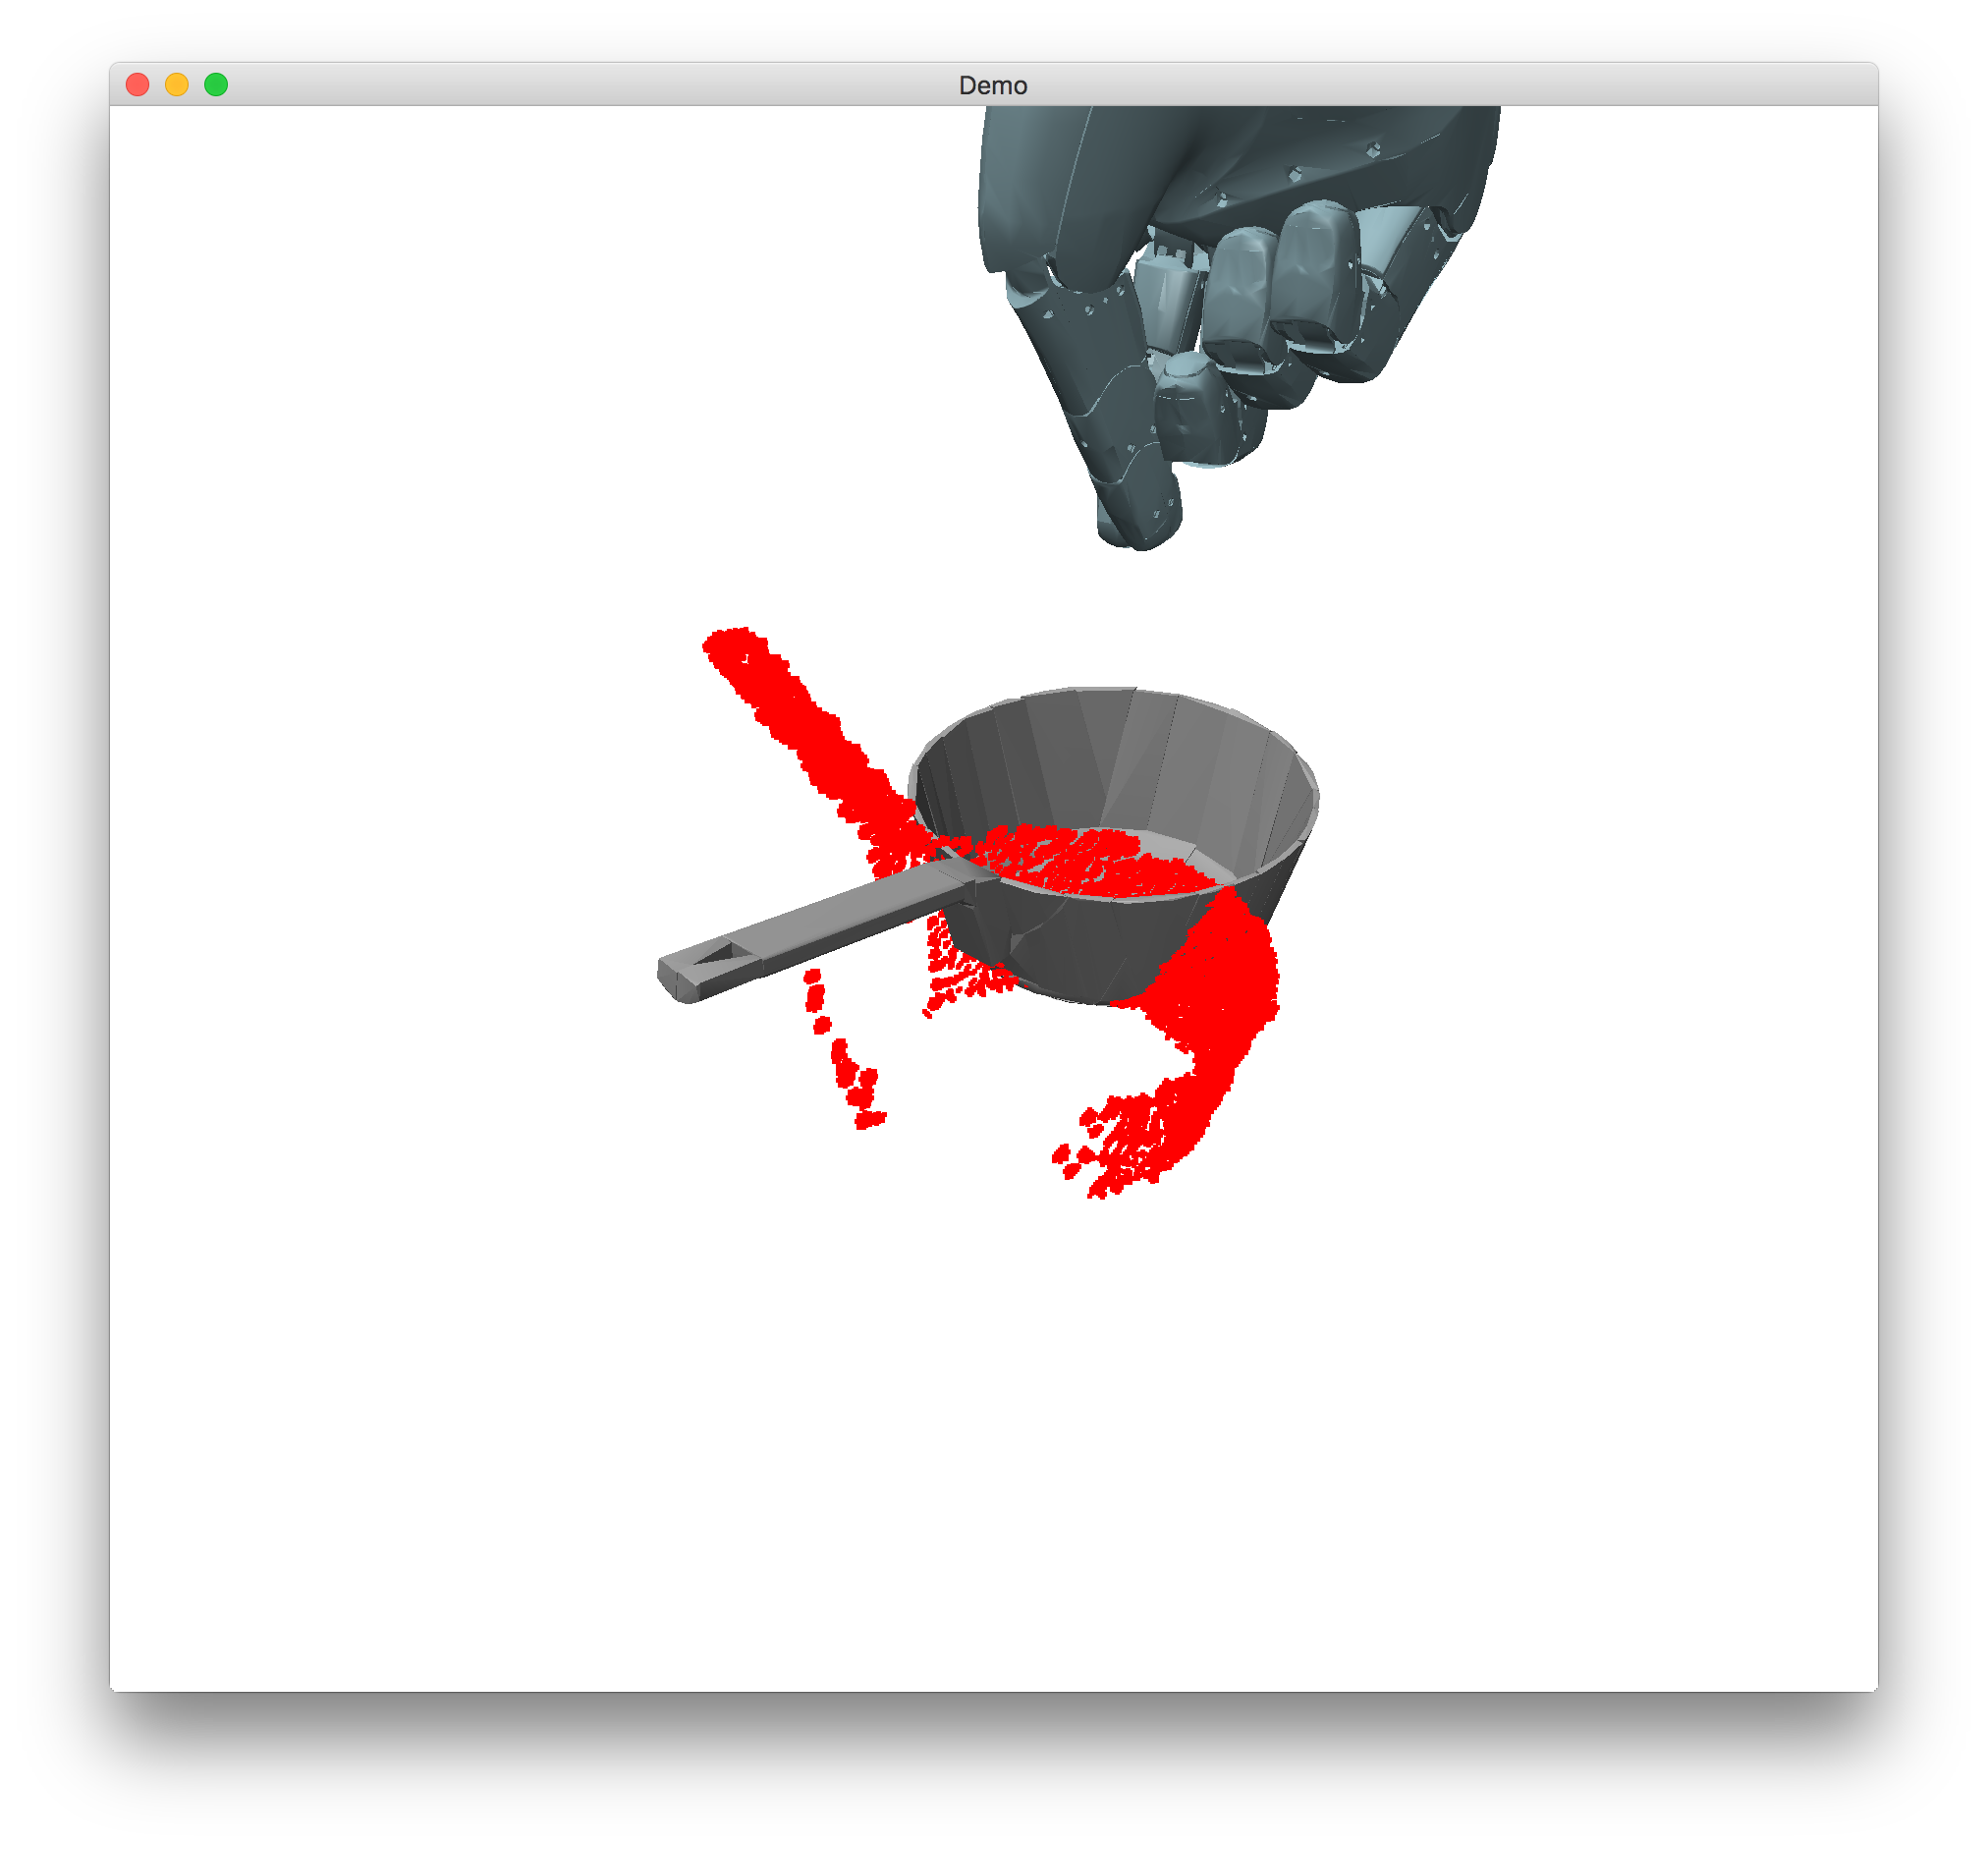
\includegraphics[width=0.24\textwidth]{images/Pan4_2_LFHW}\\
%%
\includegraphics[width=0.96\textwidth]{images/key-to-eval-training}\\
%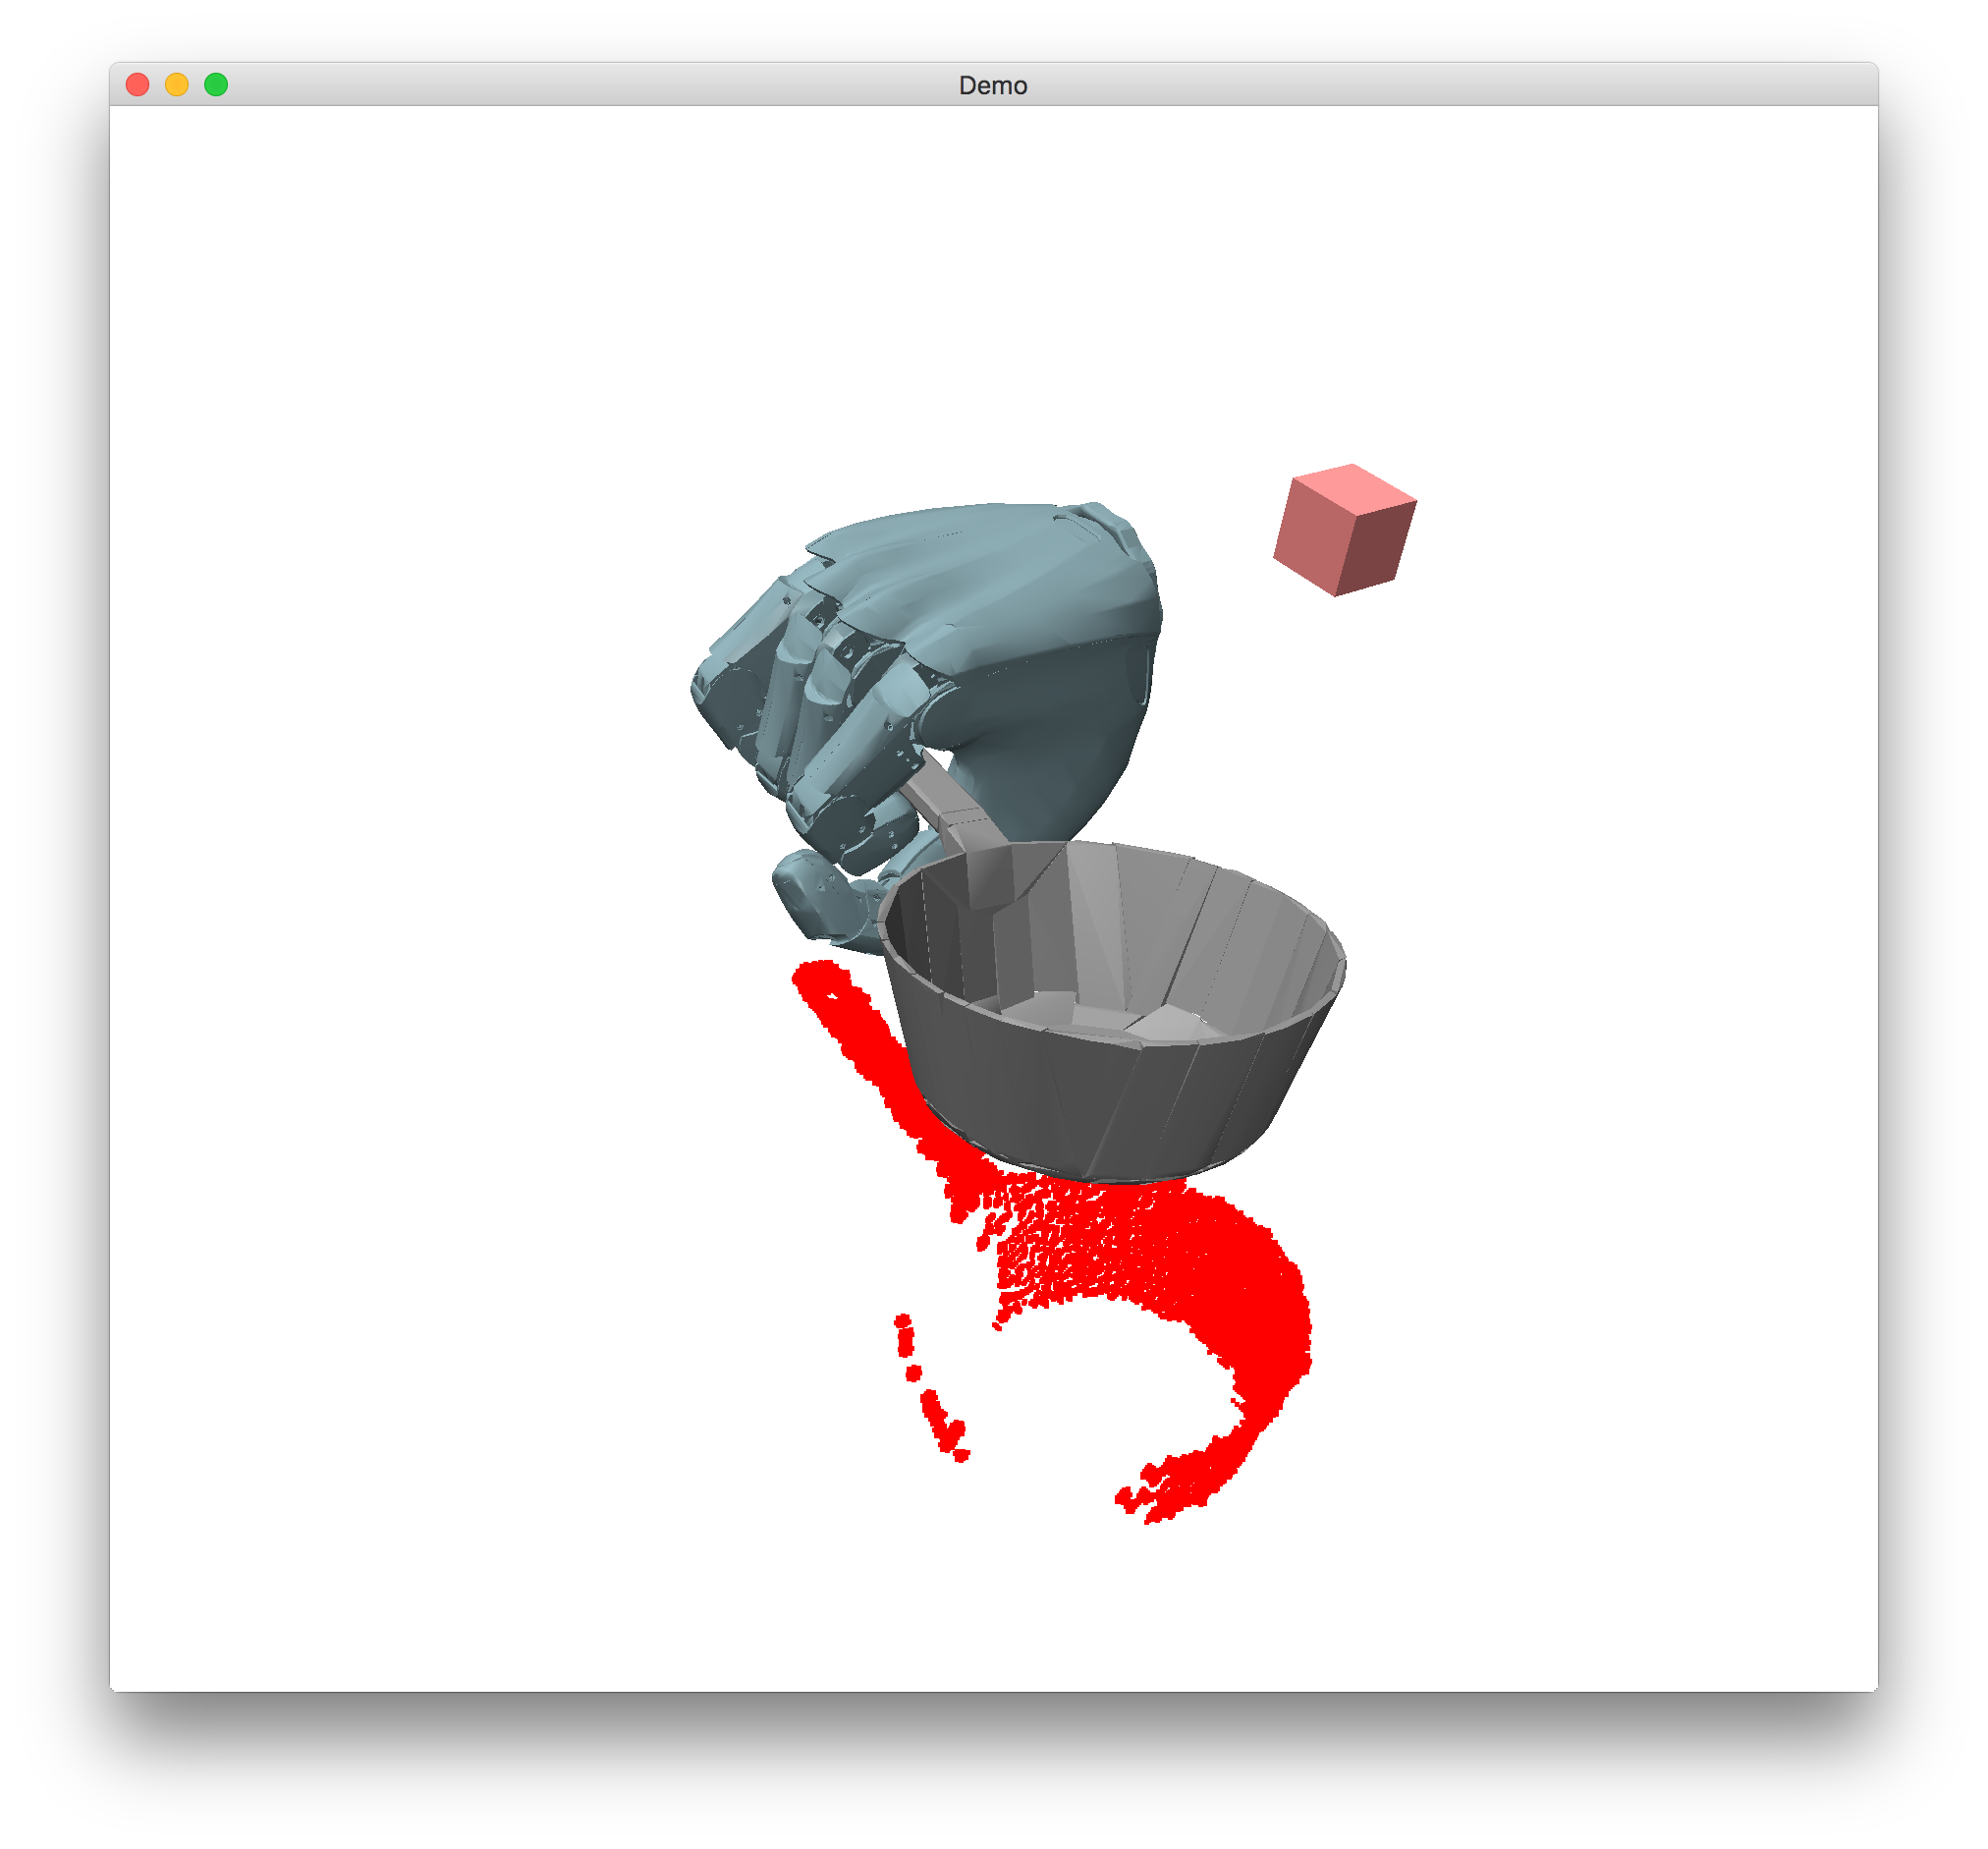
\includegraphics[width=0.24\textwidth]{images/Pan4_HFLW}
%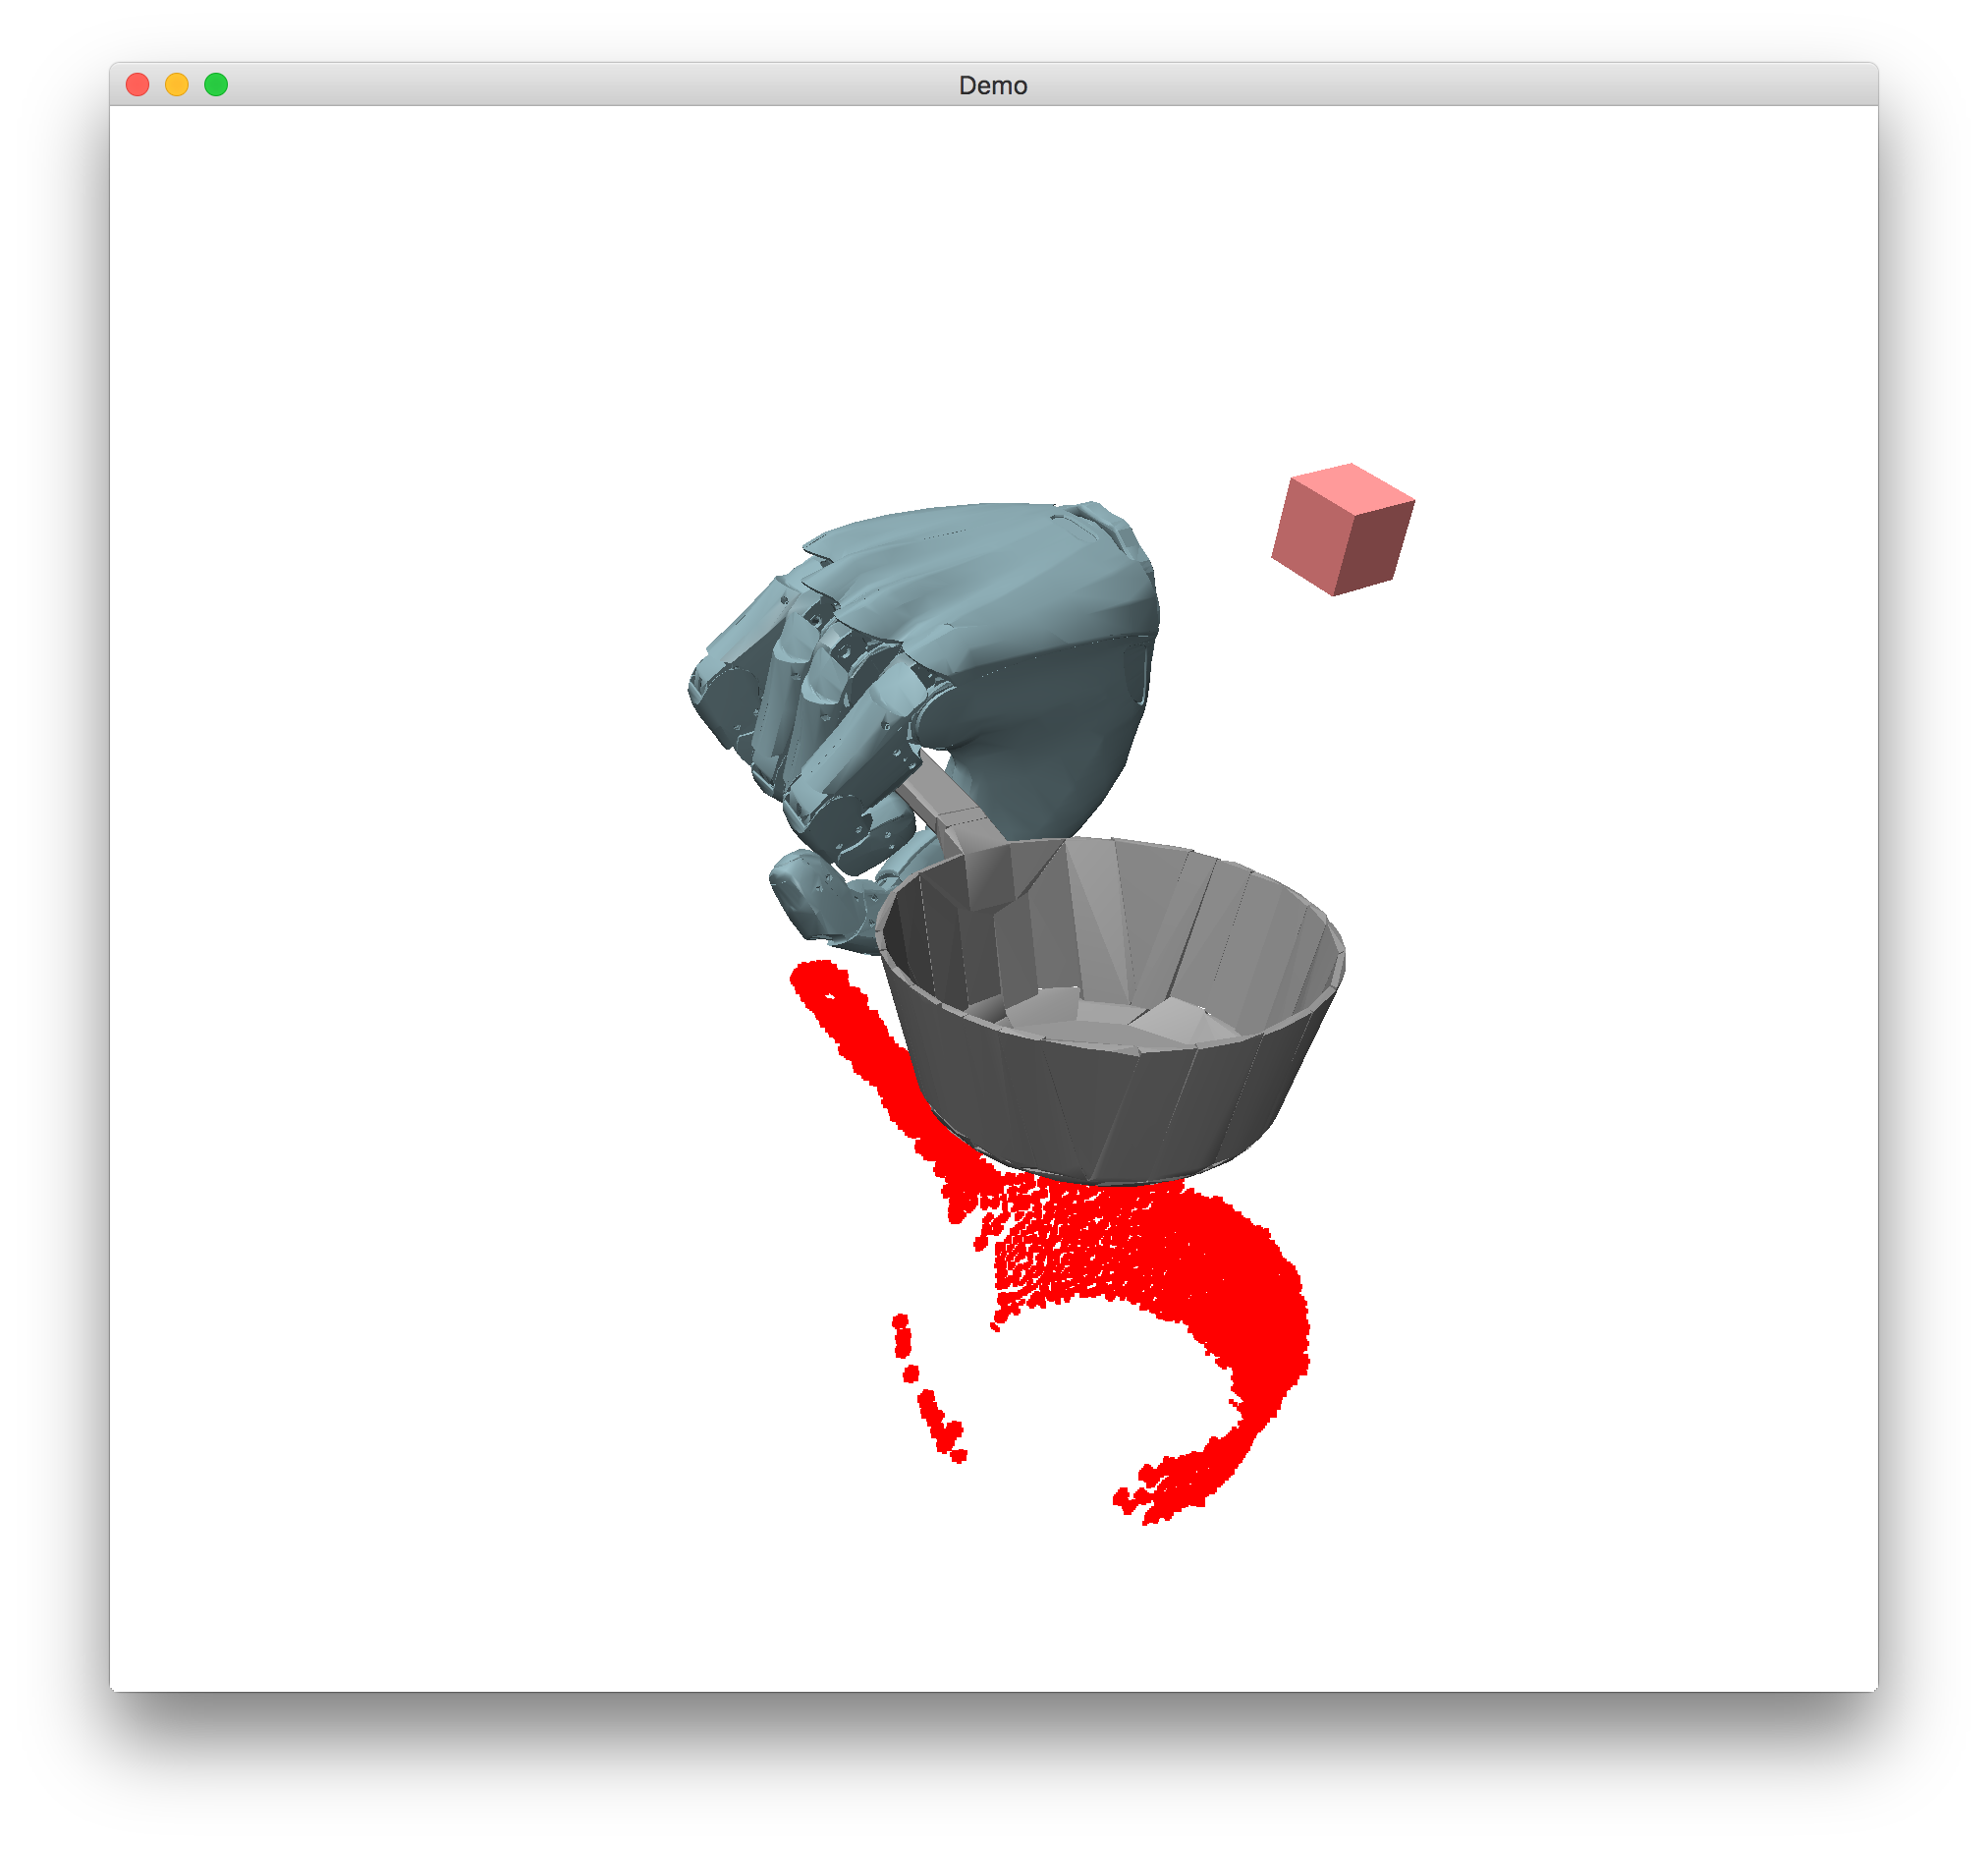
\includegraphics[width=0.24\textwidth]{images/Pan4_LFLW}
%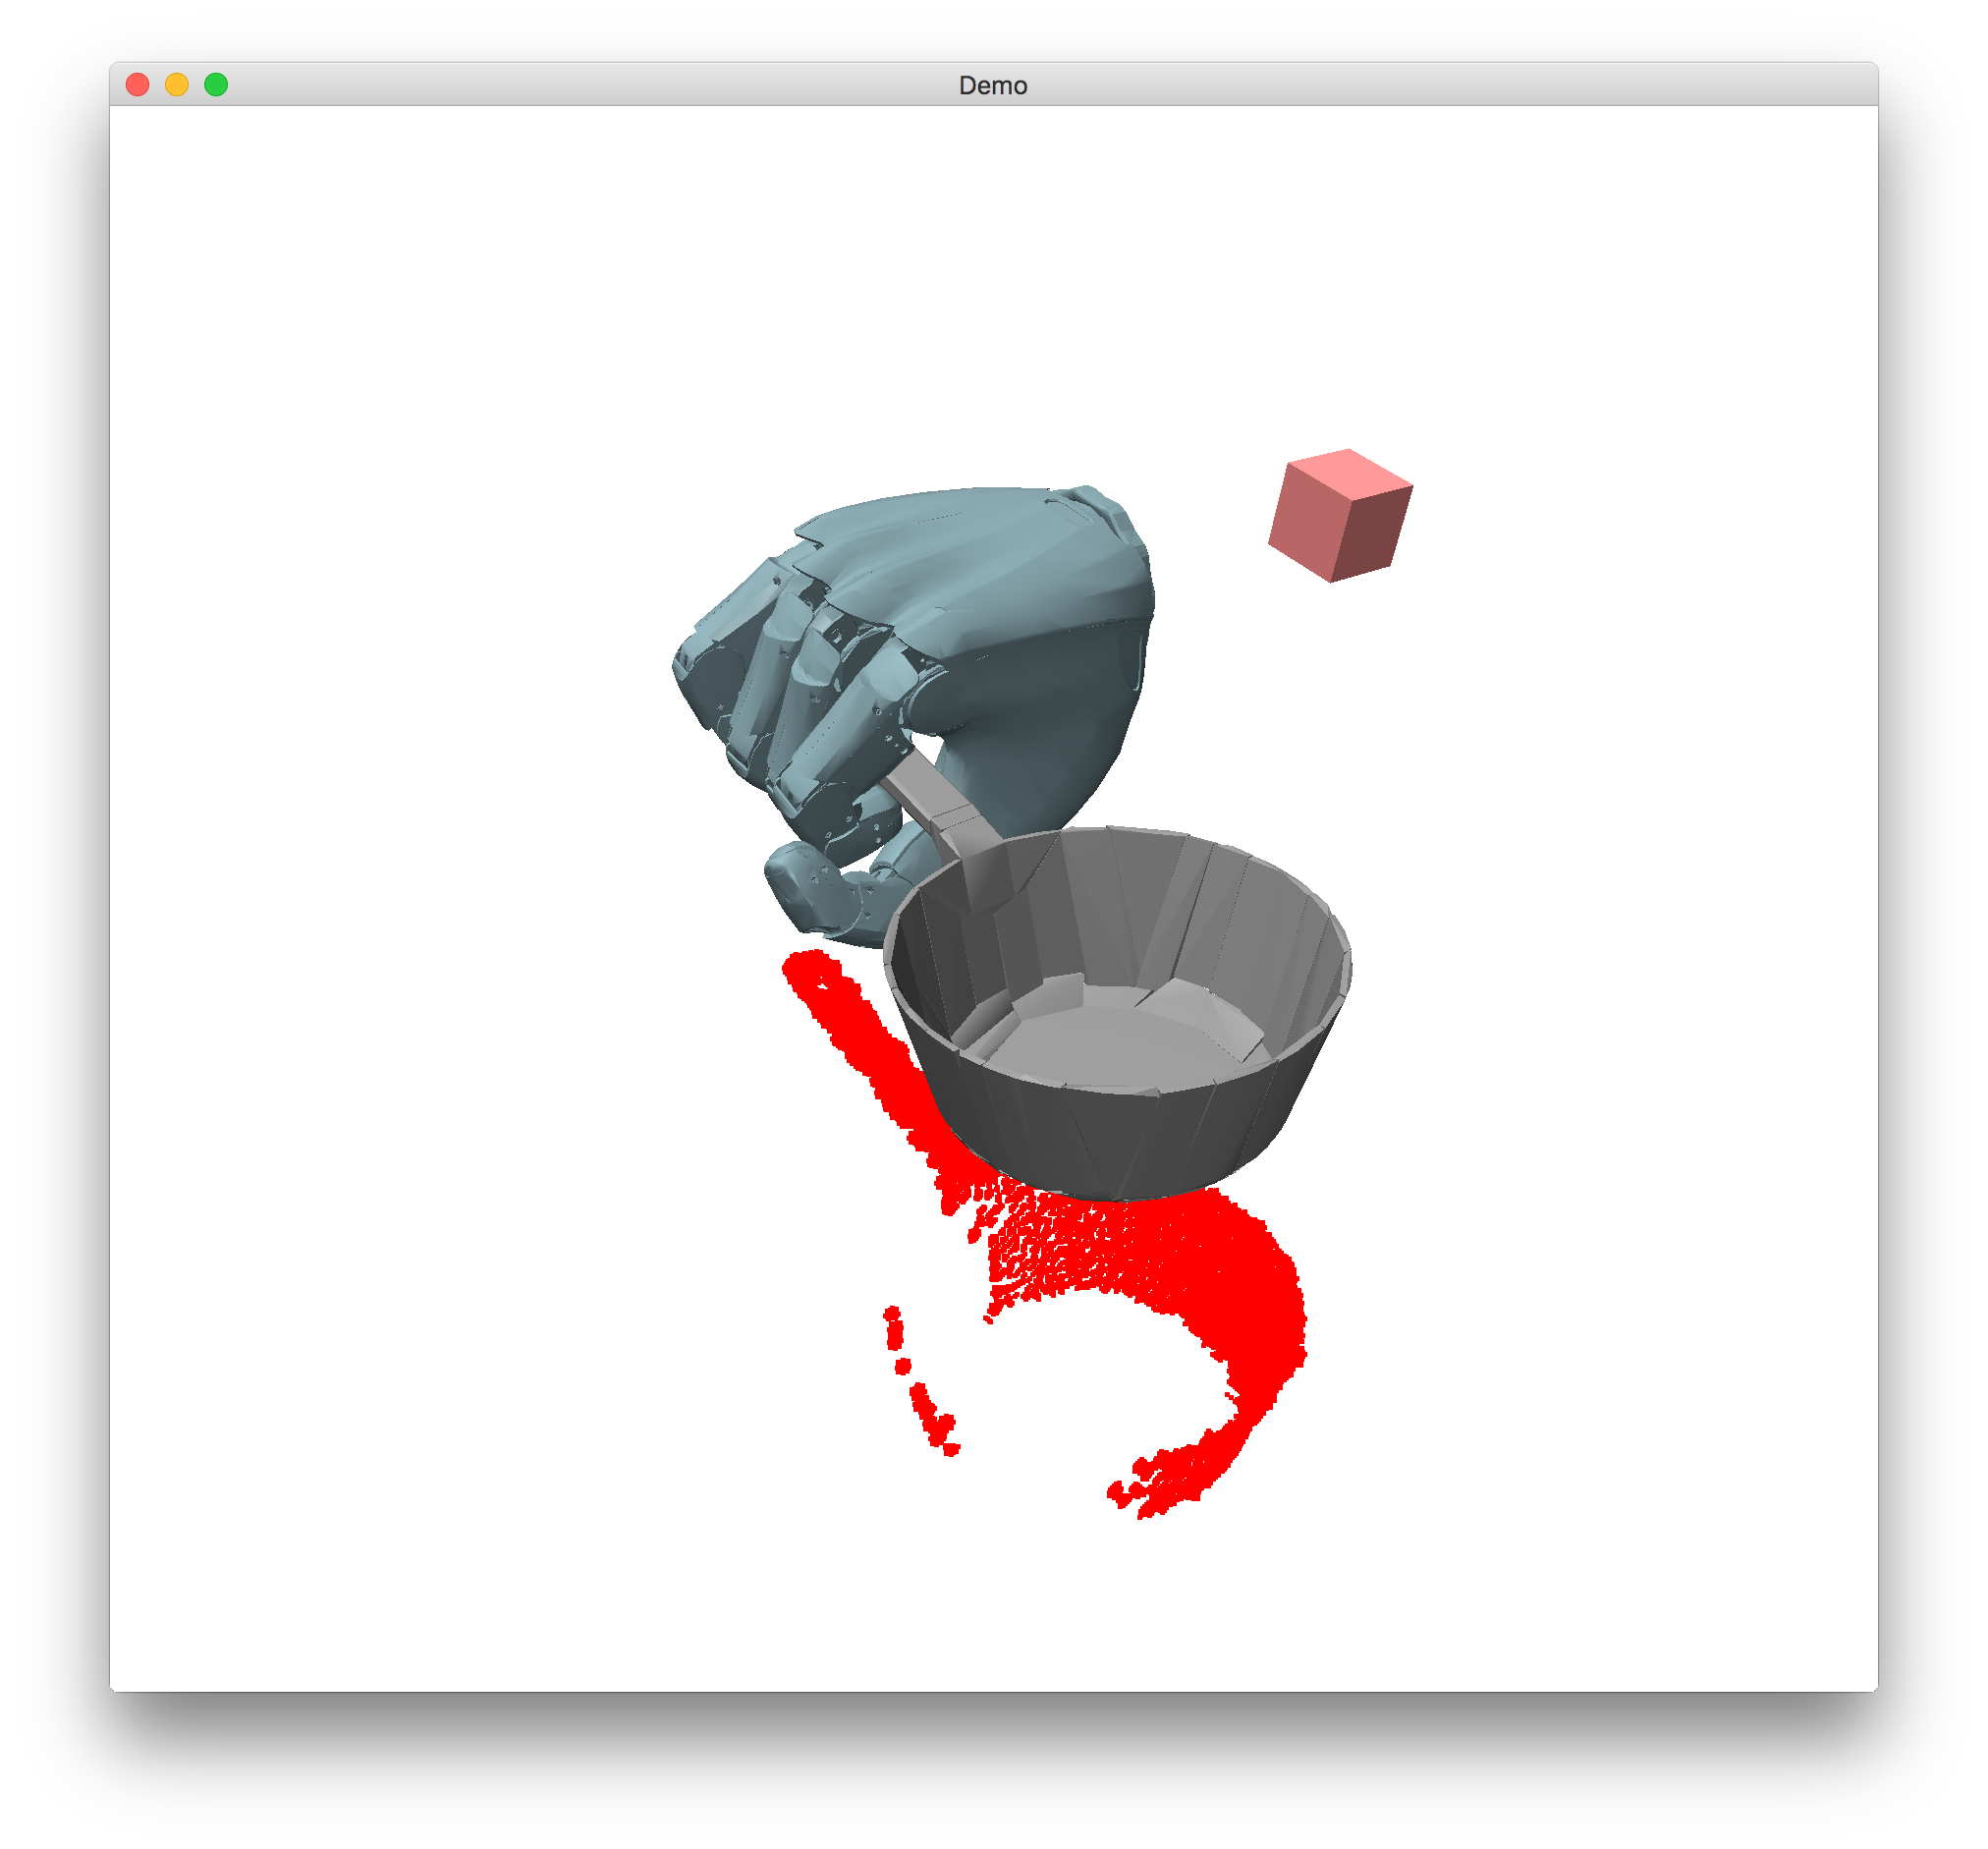
\includegraphics[width=0.24\textwidth]{images/Pan4_HFHW}
%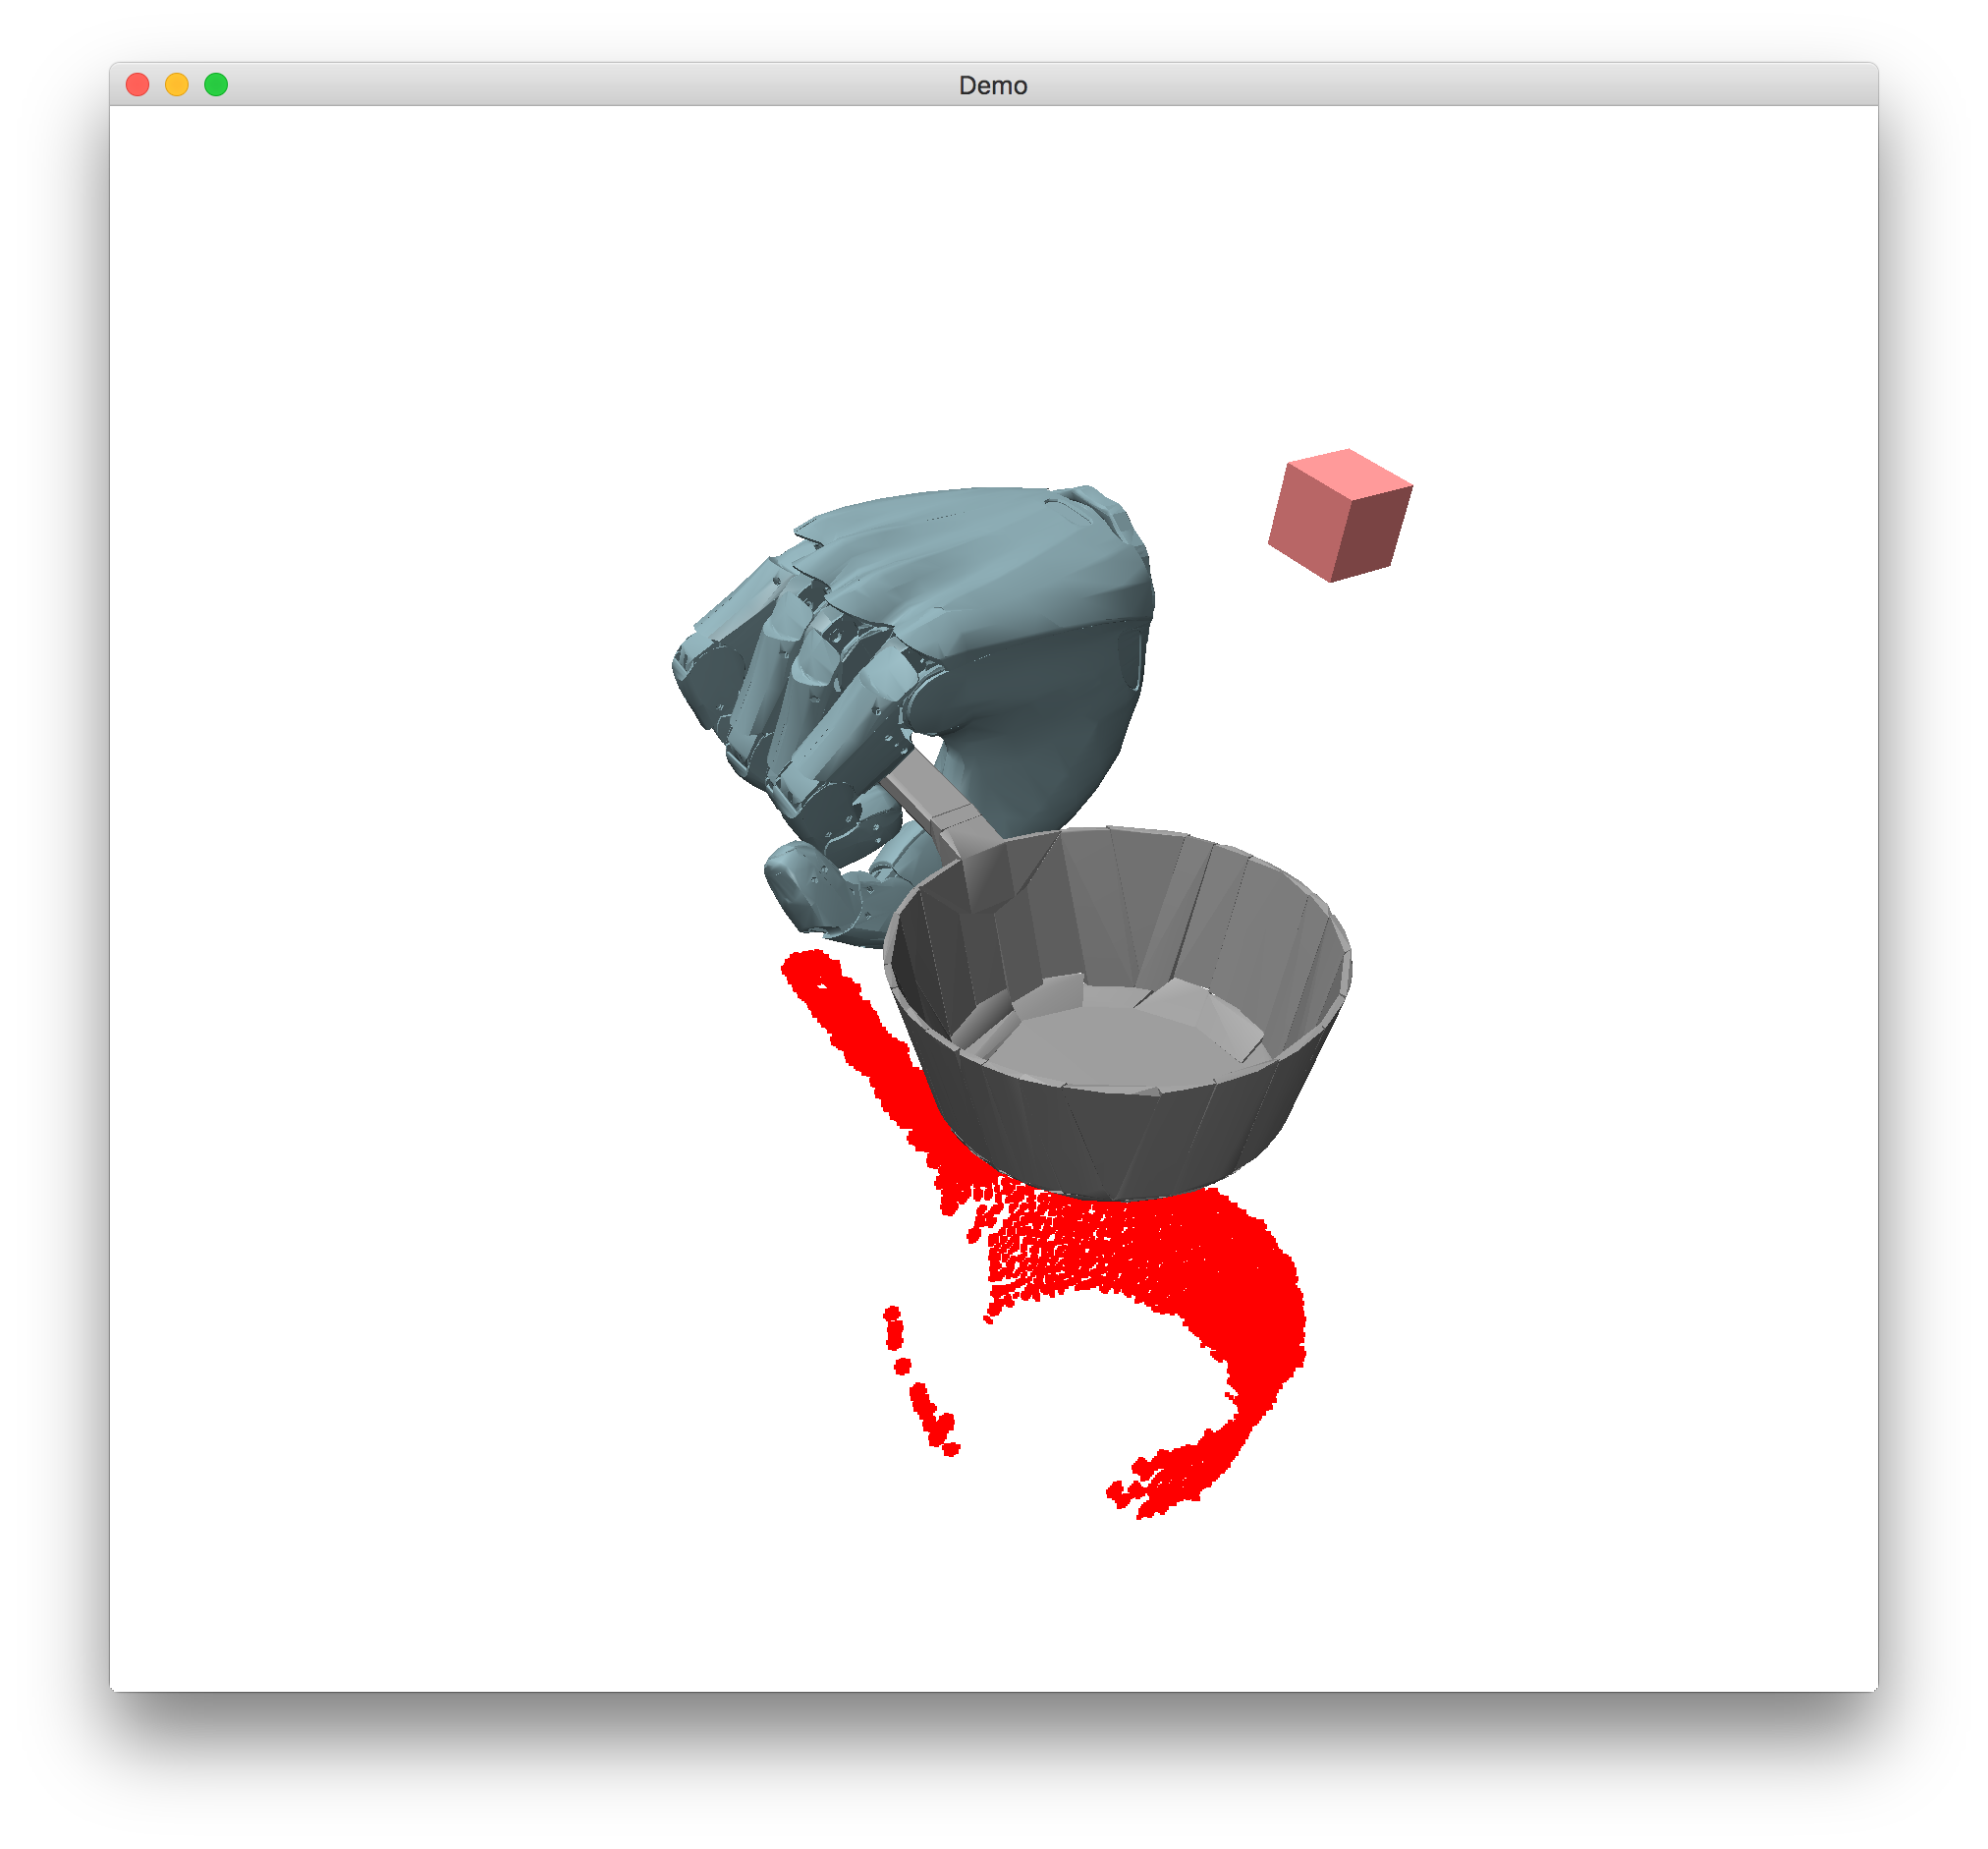
\includegraphics[width=0.24\textwidth]{images/Pan4_LFHW}
\caption{Training a robust evaluation model. (Top row) The same pinch grasp, executed on the same object, with varying friction and mass parameters. (Bottom row) A more robust power grasp, executed on the same object, with the same variation in friction and mass. \label{fig:evaluative-training}}
\end{figure}

\subsection{Training methodology}
A total of 441,312 grasps in 7,311 scenes, comprising equal numbers of successes and failures, were used to train the architecture presented in the previous section. The data set was balanced by randomly eliminating excess failure grasps, as the underlying success rate across all candidate grasps was 48\%. We used the ADAM optimiser with learning rate 0.001 and a dropout rate of 0.3. We performed early stopping.